\chapter{Geração do mapa}

A posição do robô no mapa em cada instante é representada por um ponto no plano cartesiano e por um ângulo, que indica para qual sentido o robô está orientado. Esse ponto no plano indica onde está o centro de movimento do robô, que é o ponto médio entre as duas rodas.

Neste projeto, a determinação do deslocamento do robô é determinada primariamente pelos encoders presentes cada roda. O acelerômetro e o giroscópio são utilizados para aumentar a confiabilidade dos cálculos de deslocamento, principalmente em caso de escorregamento das rodas.

Na próxima seção será explicada a teoria da determinação do deslocamento, velocidade e aceleração do centro de movimento do robô a partir das leituras dos encoders em cada instante. Na seção \ref{sec:teoria_acel_giro} será explicitada a forma como as leituras do acelerômetro e giroscópio serão utilizadas para aumentar a exatidão das medições.

Na Figura \ref{fig:robo} está presente um esquema básico do robô visto de cima e virado com a frente para a direita. Na figura estão presentes os nomes das variáveis que são utilizadas nos cálculos posteriores. As medidas $R$, $R_D$ e $R_E$ representam os raios de um movimento circular uniforme descrito pelo robô, supondo que e roda esquerda esteja se deslocando mais do que a direita. Esse aspecto será melhor explicado nas seções seguintes. 

\begin{figure}[H]
  \centering
  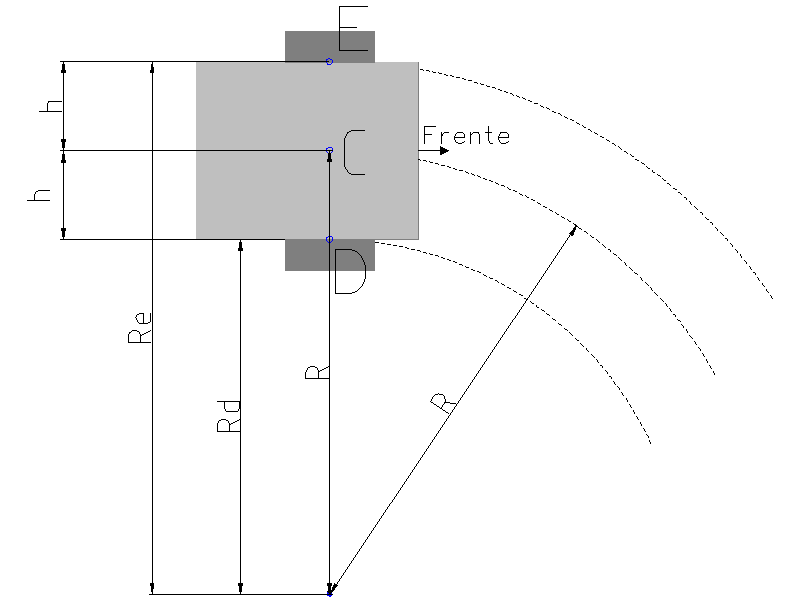
\includegraphics[width=0.8\textwidth, keepaspectratio]{./figuras/robo/robo.png}
  \caption{Representação básica do robô em movimento circular uniforme (visão superior).}
  \label{fig:robo}
\end{figure}

Um aspecto importante a ressaltar é que o sistema de coordenadas do Processing (a biblioteca usada para desenhar o mapa 2D na interface gráfica) possui o eixo Y invertido. Portanto, os ângulos crescem no sentido horário, e não no anti-horário como seria o convencional. Essa convenção do Processing (ângulos que crescem em sentido horário) é utilizada integralmente no escopo deste projeto.

\section{Encoders}

Cada encoder fornece uma medida de contagem de pulsos por volta a cada intervalo de amostragem, e isso permite calcular o deslocamento de cada roda. A partir dessas informações, dois dados importantes podem ser determinados a respeito do deslocamento do centro de movimento do robô: o deslocamento linear (distância absoluta percorrida) e o angular (variação do ângulo de orientação do robô).

Na Figura \ref{fig:roda_encoder} está presente um representação básica de uma roda, acoplada a um encoder. Os números da figura são utilizados como índices nos cálculos explicitados posteriormente.

\begin{figure}[H]
  \centering
  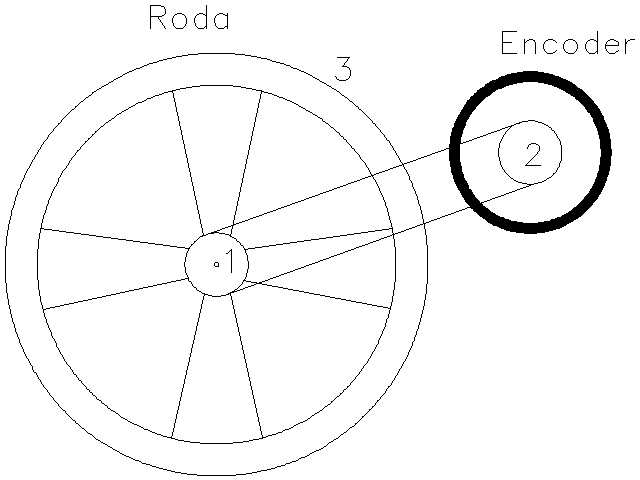
\includegraphics[width=0.5\textwidth, keepaspectratio]{./figuras/robo/roda_encoder.png}
  \caption{Representação de uma roda acoplada a um encoder.}
  \label{fig:roda_encoder}
\end{figure}

\subsection{Deslocamento de cada roda}

Um princípio importante utilizado nos cálculos é a relação entre o deslocamento $\Delta x$ ao redor de uma circunferência (de raio $R$) e a variação do ângulo $\Delta \theta$:

\begin{equation}
  \Delta x = R \cdot \Delta \theta
  \label{eq:deslocamento_circunferencia}
\end{equation}

Nos cálculos a seguir, faz-se uso do índice 1 para o eixo da roda, 2 para o eixo do encoder e 3 para a própria roda, de acordo com a figura \ref{fig:roda_encoder}. Para determinar a distância percorrida pela roda, deve-se considerar a circunferência do eixo da roda ($C_1$), a circunferência do eixo do encoder ($C_2$) e a circunferência da roda ($C_3$).

O acoplamento do eixo do encoder com o eixo da roda é feita por uma correia de borracha, e portanto considera-se que o deslocamento ($ \Delta x_1$) na superfície do eixo da roda é igual ao deslocamento ($ \Delta x_2$) na superfície do eixo do encoder. Pode-se, com isso, calcular:

\begin{eqnarray*}
   \Delta x_1 =  \Delta x_2 \rightarrow \Delta \theta_1 R_1 = \Delta \theta_2 R_2 \rightarrow \Delta \theta_1 \frac{C_1}{2 \pi} = \Delta \theta_2 \frac{C_2}{2 \pi} 
\end{eqnarray*}

\begin{equation}
  \Delta \theta_1 = \frac{C_2}{C_1} \cdot \Delta \theta_2
  \label{eq:theta1_theta2}
\end{equation}

Calculando-se a relação entre a contagem de pulsos do encoder ($E$) e o ângulo de rotação ($\Delta \theta_2$) do eixo do encoder, levando-se em conta que há uma contagem de $PV$ pulsos por volta:

\begin{equation}
  \Delta \theta_2 = \frac{2 \pi}{PV} \cdot E \unit{rad}
  \label{eq:E_theta2}
\end{equation}

Substituindo-se a equação \ref{eq:E_theta2} na \ref{eq:theta1_theta2}, tem-se que:

\begin{equation}
  \Delta \theta_1 = \frac{C_2}{C_1} \frac{2 \pi}{PV} \cdot E \unit{rad}
  \label{eq:theta_1}
\end{equation}

Calculando-se a relação entre a variação do ângulo do eixo da roda ($\Delta \theta_1$) e o deslocamento da roda ($\Delta x_3$):

\begin{eqnarray*}
  \Delta \theta_1 = \Delta \theta_3 \rightarrow \Delta \theta_1 =  \frac{\Delta x_3}{R_3} \rightarrow \Delta \theta_1 = \Delta x_3 \frac{2 \pi}{C_3} \rightarrow  \Delta x_3 = \Delta \theta_1 \frac{C_3}{2 \pi}
\end{eqnarray*}

Substituindo-se o valor de ($\Delta \theta_1$) da equação \ref{eq:theta_1}, obtém-se:

\begin{eqnarray*}
   \Delta x_3 = \frac{C_2}{C_1} \frac{2 \pi}{PV} \cdot E \cdot \frac{C_3}{2 \pi}
\end{eqnarray*}

\begin{empheq}[box=\fbox]{equation}
   \Delta x_3 = \frac{C_2 C_3}{PV \cdot C_1} \cdot E
  \label{eq:x_3}
\end{empheq}


Que é o valor do deslocamento da roda em função da contagem de pulsos do encoder. 

\subsubsection{Valores práticos}

Os discos do encoders instalados atualmente no robô possuem nominalmente 1800 pulsos por volta. Porém, eles estão visivelmente danificados, o que gera falhas na geração de pulsos. Na prática, os valores reais foram determinados a partir de 10 rotações dos discos, calculando-se o valor médio. A roda esquerda gera aproximadamente $PV=1708$ pulsos, e a direita $PV=1627$ pulsos por volta.

As medidas das circunferências $C_1$ (eixo da roda), $C_2$ (eixo do encoder) e $C_3$ (roda) do robô estão presentes no Apêndice \ref{cap:medidas_robo}.

\subsection{Deslocamento do centro de movimento do robô}

Como já explicitado anteriormente, o centro de movimento do robô considerado é o ponto médio entre as duas rodas. As duas variáveis para determinar em cada instante de tempo são o deslocamento linear (distância absoluta percorrida) e o angular (variação do ângulo de orientação do robô). Considerando-se que em cada instante o robô descreve um movimento circular uniforme (MCU), o raio da trajerória deve ser determinado para que os cálculos de posicionamento do robô possam ser feitos. Este raio depende do deslocamento das rodas em cada instante, e é uma importante variável que será estudada na próxima subseção.

Nos cálculos que serão explicitados a seguir, utiliza-se o índice E para a roda esquerda, C para o centro de movimento do robô e D para a roda direita.

Uma relação importante a notar a princípio é que a variação do ângulo de orientação em cada instante é igual nos três pontos: E (roda esquerda), C (centro de movimento) e D (roda direita), visto que todos estão fixos em relação à carcaça do robô. Parte-se da seguinte relação fundamental, portanto:

\begin{equation}
  \Delta \theta_E = \Delta \theta_D = \Delta \theta_C
  \label{eq:relacao_fundamental_theta}
\end{equation}



\subsubsection{Raio do movimento circular uniforme}

Para determinar o raio ($R$) descrito pelo centro de movimento do robô em sua trajetória instantânea em MCU, usa-se os dois primeiros termos da igualdade da equação \ref{eq:relacao_fundamental_theta}:

\begin{eqnarray*}
  \Delta \theta_E = \Delta \theta_D \rightarrow \frac{\Delta x_E}{R_E} = \frac{\Delta x_D}{R_D} 
\end{eqnarray*}

Sabe-se, pela Figura \ref{fig:robo}, que:
\begin{equation*}
  R_E = R + h, ~ ~ R_D = R - h
\end{equation*}

Portanto:

\begin{eqnarray*}
  \frac{\Delta x_E}{R + h} = \frac{\Delta x_D}{R - h} ~\rightarrow~ \frac{\Delta x_E}{\Delta x_D} = \frac{R + h}{R - h} ~\rightarrow~ \frac{\Delta x_E (R - h)}{\Delta x_D} = R + h 
\end{eqnarray*}
\begin{eqnarray*}
  \frac{\Delta x_E \cdot R - \Delta x_E \cdot h}{\Delta x_D} = R + h ~\rightarrow~ 
  \frac{\Delta x_E}{\Delta x_D} \cdot R - \frac{\Delta x_E}{\Delta x_D} \cdot h = R + h ~\rightarrow~ 
  \frac{\Delta x_E}{\Delta x_D} \cdot R - R = \frac{\Delta x_E}{\Delta x_D} \cdot h + h
\end{eqnarray*}
\begin{eqnarray*}
  R \left( \frac{\Delta x_E}{\Delta x_D} - 1 \right) = h \left( \frac{\Delta x_E}{\Delta x_D} + 1 \right) ~\rightarrow~
  R = h \cdot \frac{\left( \frac{\Delta x_E}{\Delta x_D} + 1 \right)}{\left( \frac{\Delta x_E}{\Delta x_D} - 1 \right)}  ~\rightarrow~
  R = h \cdot \frac{\frac{\Delta x_E + \Delta x_D}{\Delta x_D}}{\frac{\Delta x_E - \Delta x_D}{\Delta x_D}} 
\end{eqnarray*}

\begin{empheq}[box=\fbox]{equation}
  R = h \cdot \frac{\Delta x_E + \Delta x_D} {\Delta x_E - \Delta x_D}
  \label{eq:R}
\end{empheq}

Vê-se que o raio $R$ do movimento circular uniforme em cada instante depende do deslocamento de cada roda ($\Delta x_E$ e $\Delta x_D$) e da distãncia $h$ entre as rodas e o centro de movimento do robô.


\subsubsection{Deslocamento linear} 

Para calcular o deslocamento linear do centro de movimento do robô, usa-se os dois últimos termos da equação \ref{eq:relacao_fundamental_theta}. Vale ressaltar que poderiam ser escolhidos também o primeiro e o último termos, pois o resultado obtido seria idêntico. Tem-se que:

\begin{eqnarray*}
  \Delta \theta_D = \Delta \theta_C \rightarrow \frac{\Delta x_D}{R_D} = \frac{\Delta x_C}{R} 
\end{eqnarray*}

Mas:
\begin{equation*}
  R_D = R - h
\end{equation*}

Portanto:
\begin{eqnarray*}
  \frac{\Delta x_D}{R - h} = \frac{\Delta x_C}{R} ~\rightarrow~ x_D = x_C \cdot \frac{R - h}{R} 
\end{eqnarray*}

Substituindo-se o valor de $R$ da equação \ref{eq:R}:
\begin{eqnarray*}
  \Delta x_D = \Delta x_C \left[ \frac{h \cdot \frac{\Delta x_E + \Delta x_D}{\Delta x_E - \Delta x_D} - h}{h \cdot \frac{\Delta x_E + \Delta x_D}{\Delta x_E - \Delta x_D}} \right]
\end{eqnarray*}

Dividindo-se o numerador e denominador do segundo termo por $h$:
\begin{equation*}
  \Delta x_D = \Delta x_C \left[ \frac{\frac{\Delta x_E + \Delta x_D}{\Delta x_E - \Delta x_D} - 1}{\frac{\Delta x_E + \Delta x_D}{\Delta x_E - \Delta x_D}} \right]
\end{equation*}

Multiplicando-se o numerador e denominador do segundo termo por $\frac{\Delta x_E - \Delta x_D}{\Delta x_E + \Delta x_D}$:

\begin{equation*}
  \Delta x_D = \Delta x_C \left[1 - \frac{\Delta x_E - \Delta x_D}{\Delta x_E + \Delta x_D} \right] ~\rightarrow~
  \Delta x_D = \Delta x_C \left[\frac{(\Delta x_E + \Delta x_D) - (\Delta x_E - \Delta x_D)}{\Delta x_E + \Delta x_D} \right] 
\end{equation*}
\begin{equation*}
  \Delta x_D = \Delta x_C \cdot \left[ \frac{2 \Delta x_D}{\Delta x_E + \Delta x_D} \right] ~\rightarrow~
  \Delta x_C = \frac{\Delta x_D}{\left(\frac{2 \Delta x_D}{\Delta x_E + \Delta x_D} \right)}
\end{equation*}

\begin{empheq}[box=\fbox]{equation}
  \Delta x_C = \frac{\Delta x_E + \Delta x_D}{2}
  \label{eq:desloc_linear}
\end{empheq}

Notas-se que o deslocamento linear do centro de movimento do robô ($\Delta x_C$) é uma média simples dos dois deslocamentos lineares das rodas. Vê-se que ele não depende do raio de deslocamento nem da distância entre as duas rodas.


\subsubsection{Deslocamento angular}

O deslocamento angular ($\Delta \theta_c$) do centro de movimento do robô em cada instante pode ser calculado a partir do deslocamento linear e do raio do movimento circular uniforme. Usando-se a relação da equação \ref{eq:deslocamento_circunferencia}, tem-se que:


\begin{empheq}[box=\fbox]{equation}
  \Delta \theta_c = \frac{\Delta x_C}{R}
  \label{eq:desloc_angular}
\end{empheq}


Onde $\Delta x_C$ é o deslocamento linear do robô (equação \ref{eq:desloc_linear}) e $R$ é o raio do movimento circular uniforme (equação \ref{eq:R}). 

\subsubsection{Casos especiais}

Há dois casos especiais que devem ser considerados no cálculo do deslocamento (a partir dos dados dos encoders) do centro de movimento do robo. O primeiro é quando as duas rodas têm deslocamento igual ($\Delta x_E = \Delta x_D$). O raio do movimento circular (equação \ref{eq:R}) neste caso é:

\begin{equation}
  R = h \cdot \frac{\Delta x_E + \Delta x_D} {\Delta x_E - \Delta x_D} = h \cdot \frac{2 \cdot \Delta x_E}{0} \rightarrow \infty
  \label{eq:caso_especial1_R}
\end{equation}


O raio tende a infinito, o que implica que o deslocamento angular (equação \ref{eq:desloc_angular}) seja:

\begin{equation}
  \Delta \theta_c = \frac{\Delta x_C}{R} = \frac{\Delta x_C}{\infty} \rightarrow 0
  \label{eq:caso_especial1_theta}
\end{equation}

Já o deslocamento linear (equação \ref{eq:desloc_linear}) é:

\begin{equation}
  \Delta x_C = \frac{\Delta x_E + \Delta x_D}{2} = \frac{2 \Delta x_E}{2} = \Delta x_E
  \label{eq:caso_especial1_x}
\end{equation}

Isso corresponde à realidade, uma vez que quando as rodas têm deslocamentos iguais o robô está se deslocando sem fazer curvas. Não há deslocamento angular, portanto, e o deslocamento linear do centro de movimento é igual ao deslocamento de cada roda.

O segundo caso especial ocorre quando os deslocamento têm módulos iguais, porêm sentidos contrários (ou seja, $\Delta x_E = - \Delta x_D$). O raio nesse caso é:

\begin{equation}
  R = h \cdot \frac{\Delta x_E + \Delta x_D} {\Delta x_E - \Delta x_D} = h \cdot \frac{\Delta x_E - \Delta x_E}{\Delta x_E + \Delta x_E} = 0
    \label{eq:caso_especial2_R}
\end{equation}


O deslocamento linear (equação \ref{eq:desloc_linear}) é:

\begin{equation}
  \Delta x_C = \frac{\Delta x_E + \Delta x_D}{2} = \frac{\Delta x_E - \Delta x_E}{2} = 0
  \label{eq:caso_especial2_x}
\end{equation}

Esse valor corresponde à realidade, pois quando as rodas se deslocam em sentidos contários, e na mesma quantidade, o centro de movimento do robô não se desloca linearmente, mas apenas muda seu ângulo.
Usando-se a equação \ref{eq:desloc_angular}, tenta-se calcular o valor do deslocamento angular:

\begin{equation}
  \Delta \theta_c = \frac{\Delta x_C}{R} = \frac{0}{0}
  \label{eq:caso_especial2_theta}
\end{equation}

O valor obtido é indeterminado quando usa-se essa equação. Porém, analisando-se a natureza deste caso especial, pode ser notado que há um movimento circular cujo centro é o ponto médio entre as rodas (que é o centro de movimento do robô). O raio do MCU é a distância $h$ entre uma roda e o centro do robô, e o deslocamento ao longo da circunferência é o deslocamento de qualquer uma uma das rodas. Portanto, a equação \ref{eq:deslocamento_circunferencia} pode ser utilizada, isolando-se a variável $\theta$, para determinar o deslocamento angular do robô:

\begin{equation}
  \Delta \theta_c = \frac{\Delta x_E}{h}
  \label{eq:caso_especial2_theta2}
\end{equation}

\subsubsection{Considerações sobre a notação utilizada}

A notação utilizada no decorrer do texto para representar o estado de uma variável em certo instante discreto de tempo é um número subscrito entre parênteses. Por exemplo, a posição $\overrightarrow{P}$ do robô em um instante de tempo $n$ é representado por:$\overrightarrow{P}_{(n)}$. 

Outro aspecto presente no decorrer do texto, que vale ser ressaltado para que haja melhor entendimento das demostrações, é o fato de que $\Delta x_{(n)}$ é o deslocamento absoluto do robô no intervalo de tempo discreto de $(n-1)$ até $n$.

%\begin{equation}
%  \Delta x_{(n)} = x_{(n)} - x_{(n - 1)}
%  \label{eq:delta_x}
%\end{equation}
%
%Sendo que $\Delta x_{(n)}$ é o deslocamento do robô do intervalo $(n-1)$ até $n$.

\subsubsection{Velocidade e aceleraçao}

A velocidade e aceleração lineares do centro de movimento do robô podem ser calculadas por derivação numérica do deslocamento e velocidade em cada intervalo de tempo. Em cada intervalo discreto $n$:

\begin{equation}
  v_{c (n)} = \frac{\Delta x_{c (n)} }{t_{(n)} - t_{(n-1)}}
  \label{eq:velocidade_encoders}
\end{equation}

\begin{equation}
  a_{c (n)} = \frac{v_{c (n)} - v_{c (n-1)}}{t_{(n)} - t_{(n-1)}}
  \label{eq:aceleracao_encoders}
\end{equation}


A velocidade e aceleração angulares podem ser também obtidas por derivação numérica, considerando-se que o raio do movimento circular uniforme do robô é constante dentro do intervalo considerado. Em cada intervalo discreto $n$:

\begin{equation}
  \omega_{c (n)} = \frac{\Delta \theta_{c (n)} }{t_{(n)} - t_{(n-1)}}
  \label{eq:omega_encoders}
\end{equation}

\begin{equation}
  \alpha_{c (n)} = \frac{\omega_{c (n)} - \omega_{c (n-1)}}{t_{(n)} - t_{(n-1)}}
  \label{eq:alpha_encoders}
\end{equation}


\section{Acelerômetro e giroscópio}
\label{sec:teoria_acel_giro}

O acelerômetro e o giroscópio são utilizados para aumentar a confiabilidade dos dados de deslocamento do robô em caso de escorregamento das rodas.

Como definido na seção \ref{sec:codificacao_mensagens}, é recebido um valor de 2 bytes para cada eixo do acelerômetro. A faixa de funcionamento do acelerômetro está configurada em $\pm 2$ g, logo a sensibilidade pelo \textit{datasheet} é de 16384 LSB/g. Portanto, o valor de aceleração pode ser obtido pela fórmula:

\begin{equation}
  a = \frac{valorMedido}{16384} \cdot g \unit{m/s^2}
  \label{eq:acel}
\end{equation}

Onde g é a aceleração da gravidade ($9,80665 \unit{m/s^2}$). 

Para cada eixo do giroscópio, também e obtido um valor de 2 bytes. A faixa de funcionamento do giroscópio está configurada em $\pm 250$ graus/s, logo a sensibilidade pelo \textit{datasheet} é de 131 LSB/(graus/s). Portanto, o valor de velocidade angular pode ser obtida pela fórmula:

\begin{equation}
  \omega = \frac{valorMedido}{131} \unit{graus/s} = \frac{\pi}{180} \cdot \frac{valorMedido}{131} \unit{rad/s}
  \label{eq:giro}
\end{equation}


A princípio, apenas o eixo Y do acelerômetro (voltado para trás do robô) e o eixo Z do giroscópio (posicionado no sentido baixo/cima, e com ângulos crescentes no sentido anti-horário) serão utilizados para mapeamento, visto que os dados poderão ser dessa forma comparados facilmente com os dados obtidos pelos encoders. Na Figura \ref{fig:eixos_acel_giro} está explicitada a disposição dos eixos do acelerômetro e giroscópio, extraída do \textit{datasheet} do MPU-6050. Para que uma comparação de acelerações (encoders \textit{vs} acelerômetro) e velocidades angulares (encoders \textit{vs.} giroscópio) seja realizada, o circuito integrado deve ser posicionado no centro de movimento do robô (ponto médio entre as rodas).

\begin{figure}[H]
	\centering
	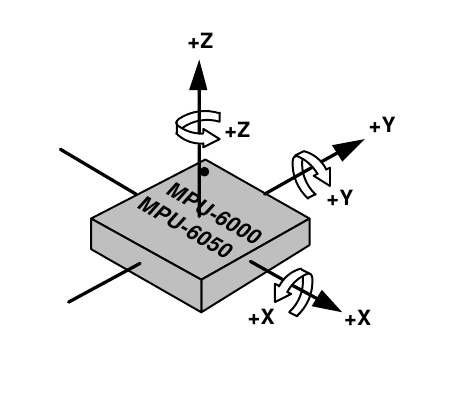
\includegraphics[width=0.7\textwidth]{./figuras/hardware/eixos_mpu.png}
	\caption{Eixos do acelerômetro e giroscópio.}
	\fonte{Datasheet do MPU-6050}
	\label{fig:eixos_acel_giro}
\end{figure}

Na prática, observou-se que o acelerômetro e o giroscópio possuem um \textit{offset} inicial, mesmo com o robô estando parado. O valor desse \textit{offset} deve ser descontado de todas as medidas obtidas para que os valores finais correspondam à realidade. Outro aspecto a ressaltar é que como o eixo Y do acelerômetro é voltado para trás do robô, os valores devem ser utilizado com sinal invertido. O eixo Z do giroscópio também deve ser utilizado com o sinal trocado, pois (como explicitado no início do capítulo) o sistema de coordenadas utilizado neste projeto implica em que os ângulos crescem em sentido horário.

Para determinar a velocidade e deslocamento lineares a partir dos dados do acelerômetro, efetua-se uma integração numérica (simples e dupla) da aceleração linear em cada intervalo discreto $n$:

\begin{equation}
  v_{(n)} = v_{(n - 1)} + a_{(n)} \cdot (t_{(n)} - t_{(n-1)})
  \label{eq:v_acelerometro}
\end{equation}
\begin{equation}
  \Delta x_{(n)} = v_{(n)} \cdot (t_{(n)} - t_{(n-1)})
  \label{eq:x_acelerometro}
\end{equation}

Para determinar o deslocamento angular a partir dos dados do giroscópio, efetua-se uma integração numérica (simples) da velocidade angular em cada intervalo discreto $n$:

\begin{equation}
  \Delta \theta_{(n)} = \Delta \theta_{(n - 1)} + \omega_{(n)} \cdot (t_{(n)} - t_{(n-1)})
  \label{eq:theta_giroscopio}
\end{equation}


\section{Algoritmo de posicionamento}

O algoritmo proposto para determinação da posição do robô em cada instante de tempo, utilizando os vários sensores (encoders, acelerômetro e giroscópio), está explicitado nesta seção. Para cada amostra dos sensores que é recebida o algoritmo efetua os seguintes passos:

\begin{enumerate}
  \item A partir das leituras dos encoders ($\Delta x_E$ e $\Delta x_D$), usando as equações \ref{eq:desloc_linear} e \ref{eq:desloc_angular}, calcular deslocamento linear ($\Delta x_C$, em metros) e angular ($\Delta \theta_c$, em $rad$) do centro de movimento do robô.
  
  \item Derivar duas vezes o deslocamento linear ($\Delta x_C$), usando as equações \ref{eq:velocidade_encoders} e \ref{eq:aceleracao_encoders} para obter aceleração linear ($a_C$, em $m/s^2$), e derivar uma vez o deslocamento angular ($\theta_C$), usando a equação \ref{eq:omega_encoders}, para obter a velocidade angular ($\omega_C$, em $rad/s$).
  
  \item Comparar a aceleração linear ($a_C$) e a velocidade angular ($\omega_C$), obtidas com os encoders, com as leituras do acelerômetro ($a_a$) e giroscópio ($\omega_g$). Caso as diferenças dos valores passem de limiares $L_a$ e $L_\omega$ (determinados experimentalmente), é provável que um escorregamento de rodas ou falha de leitura tenha ocorrido. Especificar com base nas comparações pesos $p_{a_c}$ e $p_{a_a}$ para a aceleração linear (encoders \textit{vs.} acelerômetro) e pesos $p_{\omega_c}$ e $p_{\omega_g}$ para velocidade angular (encoders \textit{vs.} giroscópio), dando mais prioridade ao acelerômetro e giroscópio caso escorregamentos sejam detectados. Em termos formais, tem-se que:
  \label{item:pesos}
  \[
  p_{a_c} =  
  \begin{cases}
      0, & |a_C - a_a| > L_a \\
      1, & \mbox{ caso contrário} 
      \label{eq:p_ac}
  \end{cases}
  \]
   \[
  p_{a_a} =  
  \begin{cases}
      1, & |a_C - a_a| > L_a \\
      0, & \mbox{ caso contrário}
      \label{eq:p_ac}
  \end{cases}
  \]
   \[
  p_{\omega_c} =  
  \begin{cases}
      0, & |\omega_C - \omega_a| > L_\omega \\
      1, & \mbox{ caso contrário}
      \label{eq:p_ac}
  \end{cases}
  \]
  \[
  p_{\omega_g} =  
  \begin{cases}
      1, & |\omega_C - \omega_a| > L_\omega \\
      0, & \mbox{ caso contrário}
      \label{eq:p_ac}
  \end{cases}
  \]
  
  \item Calcular com base nos pesos obtidos anteriormente a aceleração linear final ($a$) e a velocidade angular final ($\omega$), de acordo com as equações \ref{eq:comb_linear_acel} e \ref{eq:comb_linear_vel_angular}.
  \begin{equation}
      a = p_{a_c} \cdot a_c + p_{a_a} \cdot a_a
      \label{eq:comb_linear_acel}
    \end{equation}
  \begin{equation}
      \omega = p_{\omega_c} \cdot \omega_c + p_{\omega_g} \cdot \omega_g
      \label{eq:comb_linear_vel_angular}
    \end{equation}    
  
  \item Usando-se as equações \ref{eq:v_acelerometro} e \ref{eq:x_acelerometro}, integrar duplamente a aceleração linear ($a$) para obter o deslocamento linear ($\bm{\Delta x}$) do robô, e a partir da equação \ref{eq:theta_giroscopio} integrar uma vez a velocidade angular ($\omega$) para obter o deslocamento angular ($\bm{\Delta \theta}$) do robô.
  
  \item A partir das equações \ref{eq:P_x} e \ref{eq:P_y} explicitadas abaixo, calcular a nova posição ($\overrightarrow{P}_{(n)}$) do robô, e a partir da equação \ref{eq:theta_n} calcular o novo ângulo $\theta_{(n)}$ do robô. Decompondo-se o vetor posição ($\overrightarrow{P}$) em suas componentes $P_x$ e $P_y$, tem-se que no intervalo discreto $n$:
    \begin{equation}
      P_{x (n)} = P_{x (n-1)} + \bm{\Delta x} \cdot \cos{(\theta_{(n-1)})}
      \label{eq:P_x}
    \end{equation}
    \begin{equation}
      P_{y (n)} = P_{y (n-1)} + \bm{\Delta x} \cdot \sin{(\theta_{(n-1)})}
      \label{eq:P_y}
    \end{equation}
    \begin{equation}
      \theta_{(n)} = \theta_{(n-1)} + \bm{\Delta \theta}
      \label{eq:theta_n}
    \end{equation}
\end{enumerate}

Um ponto importante a ressaltar é que os pesos calculados no passo \ref{item:pesos} são utilizados (a princípio) como sendo 0 ou 1. Ou seja, se escorregamentos forem detectados nas rodas os pesos $p_{a_a}$ e $p_{\omega_g}$ devem valer 1, e $p_{a_c}$ e $p_{\omega_c}$ devem valer 0. Dessa forma os dados do acelerômetro e do giroscópio são utilizados (nesses momentos específicos) em detrimento dos dados dos encoders.


\section{Sensores infra-vermelhos}

Os sensores infra-vermelhos são usados para detectar obstáculos próximos ao robô (de 30 a 150 cm de distância). Na Figura \ref{fig:robo_ir} está explicitada uma representação de um sensor infra-vermelho detectando um obstáculo. Na figura estão presentes os nomes das variáveis utilizadas nos cálculos. Como já explicado no começo do capítulo, o sistema de coordenadas utilizado nesse projeto possui o eixo Y invertido. Portanto, os ângulos crescem no sentido horário e não no anti-horário como seria o convencional. Por essa razão, o ângulo ``-theta(n)'' da figura -- que nesse caso específico está em sentido anti-horário em relação ao eixo X (horizontal) do mapa -- é negativo. O ângulo ``thetaIR'' é medido com com relação ao eixo X do robô (e não do mapa), e na figura ele é positivo pois está em sentido horário com relação a esse eixo.

\begin{figure}[H]
  \centering
  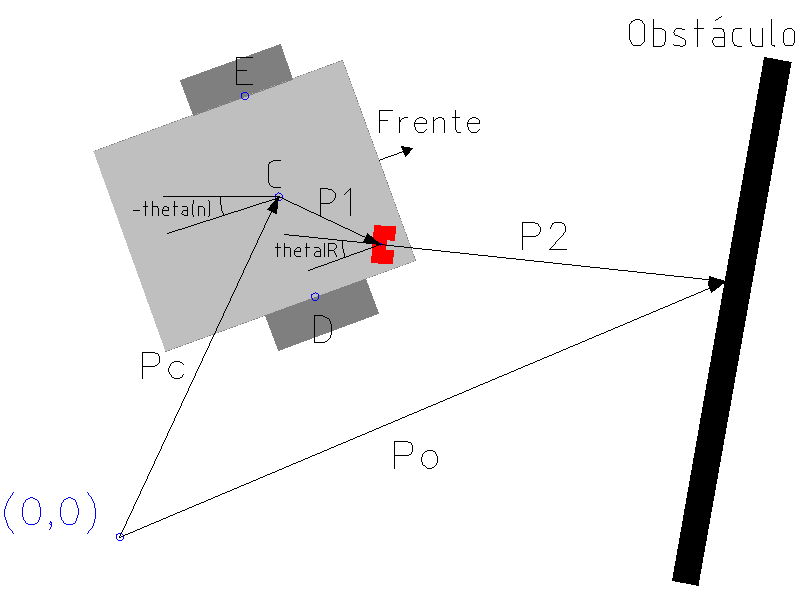
\includegraphics[width=0.8\textwidth, keepaspectratio]{./figuras/robo/robo_ir.png}
  \caption{Representação do robô e um sensor infra-vermelho detectando um obstáculo (visão superior).}
  \label{fig:robo_ir}
\end{figure}

Para obter a posição em que um obstáculo detectado está no mapa, primeiramente deve-se obter a distância entre o obstáculo e o sensor infra-vermelho. Como explicitado em \cite{bellator_2012}, o valor $x$ recebido em 1 byte do sensor pode ser convertido para a distãncia $d$ em centímetros pela fórmula (obtida por interpolação polinomial):

\begin{equation}
  d = 3,6404 \cdot 10^{-7} x^4 - 2,4435 \cdot 10^{-4} x^3 + 6,0732 \cdot 10^{-2} x^2 - 6,8962 x + 339,361
  \label{eq:IR_dist}
\end{equation}


Sendo $\overrightarrow{P_C}$ o vetor que sai da origem e vai até o centro de movimento do robô, $\overrightarrow{P_1}$ o vetor que vai do centro do robô até o sensor, e $\overrightarrow{P_2}$ o vetor que vai do sensor até o ponto do obstáculo detectado, faz-se a seguinte soma vetorial para encontrar o vetor $\overrightarrow{P_O}$, que é a posição do obstáculo no mapa:

\begin{equation}
  \overrightarrow{P_O} = \overrightarrow{P_C} + \overrightarrow{P_1} + \overrightarrow{P_2}
  \label{eq:IR_vector}
\end{equation}


O vetor $\overrightarrow{P_C}$ pode ser facilmente determinado de acordo com a equação abaixo. Sendo $\overrightarrow{P}_{(n)}$ a última posição do robô (intervalo discreto $n$):

\begin{equation}
  \overrightarrow{P_C} = \overrightarrow{P}_{(n)}
  \label{eq:IR-P_C}
\end{equation}

O vetor $\overrightarrow{P_1}$ é o vetor que vai do centro de movimento do robô até o sensor infra-vermelho. Sendo $\overrightarrow{P_{IR}}$ que vai do centro do robô até o sensor (este vetor é especificado nas configurações iniciais, supondo que o robô não esteja rotacionado), e $\theta_{(n)}$ o ângulo em que o robô está orientado em sua última posição (instante discreto $n$):


\begin{equation}
  |\overrightarrow{P_1}| = |\overrightarrow{P_{IR}}|
  \label{eq:IR-P_1_modulo}
\end{equation}
\begin{equation}
  \phi \left\{ \overrightarrow{P_1} \right\} = \phi \left\{ \overrightarrow{P_{IR}} \right\} + \theta_{(n)}
  \label{eq:IR-P_1_fase}
\end{equation}


O vetor $\overrightarrow{P_2}$ é o vetor que vai do sensor infra-vermelho até o obstáculo. Sendo $d$ a distãncia detectada pelo sensor, $\theta_{IR}$ o ângulo em que o sensor infra-vermelho está posicionado relativamente ao robô (este ângulo é especificado nas configurações iniciais, supondo que o robô não esteja rotacionado), e tendo $\theta_{(n)}$ o mesmo significado que na equação anterior:

\begin{equation}
  |\overrightarrow{P_2}| = d
  \label{eq:IR-P_2_modulo}
\end{equation}
\begin{equation}
  \phi \left\{ \overrightarrow{P_2} \right\} = \theta_{IR} + \theta_{(n)}
  \label{eq:IR-P_2_fase}
\end{equation}

\subsection{Filtragem}

Percebeu-se, nos testes realizados com o robô, que os sensores infra-vermelhos utilizados na prática provêm, esporadicamente, leituras discrepantes e que não correspondem à realidade. Portanto, certos métodos de filtragem digital foram utilizados na estação base. O primeiro filtro é um passa-faixa, que deixar passar apenas medidas que estejam entre 30cm e 150cm, que são as distâncias mínima e máxima que podem ser detectadas com exatidão pelos sensores (segundo o \textit{datasheet} do dispositivo). O segundo filtro é uma média móvel. Esse filtro pode ser ativado pelo usuário através da interface gráfica, na qual pode-se também configurar o número de períodos da média. Em alguns ambientes testados a média móvel mostrou-se adequada para melhorar a qualidade do mapa.


\chapter{Testes}
 
Nesta seção serão expostos os testes realizados na prática com o robô. Durante os testes foi possível chegar ao ponto de utilizar com sucesso o giroscópio para correção de erros de escorregamentos e de falhas de leituras dos encoders, como explicado a seguir. 

Um ponto que vale ser ressaltado, para melhor compreensão dos mapas, é que o robô sempre sai da origem (ponto marcado por (0,0) em cada mapa) e chega na posição em que está o seu ícone (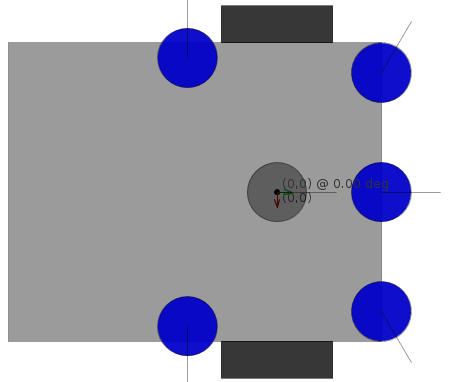
\includegraphics[scale=0.02]{figuras/robo/robo_cor_transp_cortado.png}).


%A seguir estão explicitados com maiores detalhes os processos. 


\section{Primeiro teste}


O primeiro teste bem-sucedido foi realizado utilizando com o \textit{layout} do ambiente da Figura \ref{fig:teste1_layout}. O robô fez um trajeto em sentido anti-horário no ambiente retangular, voltando à posição inicial $(0,0)$ ao final do caminho. Os encoders sofreram imprecisões nas medições em certos momentos do trajeto. No gráfico da Figura \ref{fig:teste1_giro_grafico} está explicitada uma comparação entre as velocidades angulares obtidas com os encoders e com o eixo Z do giroscópio. Vê-se que o giroscópio proveu medidas razoavelmente confiáveis no decorrer do tempo. 

Na Figura \ref{fig:teste1_mapa_encoders} está presente o mapa produzido a partir desse teste somente utilizando os dados dos encoders, e na Figura \ref{fig:teste1_mapa_encoders_giro} está presente um mapa que foi produzido utilizando as leituras do giroscópio para correção de erros (o limiar utilizado foi $L_\omega = 0.025 \unit{rad/s}$). Vê-se que o trajeto do robô pôde ser determinado com maior exatidão no segundo mapa, usando-se o giroscópio. A posição final do robô ficou próxima da origem, e o mapa ficou mais semelhante à forma retangular que corresponde à realidade. 

O acelerômetro, por outro lado, não se provou eficaz para o fim de correção de erros, ao menos não da forma como os dados estão sendo atualmente obtidos e tratados. A obtenção de dados é feita a partir de amostras instantâneas a 3.89 Hz. Na Figura \ref{fig:teste1_acel_grafico} está explicitada uma comparação (produzida a partir desse mesmo teste) das acelerações lineares obtidas com os encoders e com o eixo Y do acelerômetro. Vê-se que há grandes diferenças entre as acelerações, e que o acelerômetro provê medidas bastante discrepantes. Na Figura \ref{fig:teste1_mapa_acelerometro} está presente um mapa que foi gerado somente a partir das amostras do acelerômetro e giroscópio, exposto para fins de comparação. A trilha em azul representa o caminho que o robô supostamente percorreu de acordo com esses sensores. É visível que os resultados obtidos com o acelerômetro estão longe da realidade.

Um aspecto que vale ressaltar é que nos dois primeiros mapas foi utilizada uma filtragem de média móvel de 3 períodos para os sensores IR. No mapa da Figura \ref{fig:teste1_mapa_encoders_giro_media0}, exposto para comparação, não foi utilizada a filtragem por média móvel.


\begin{figure}[H]
	\centering
	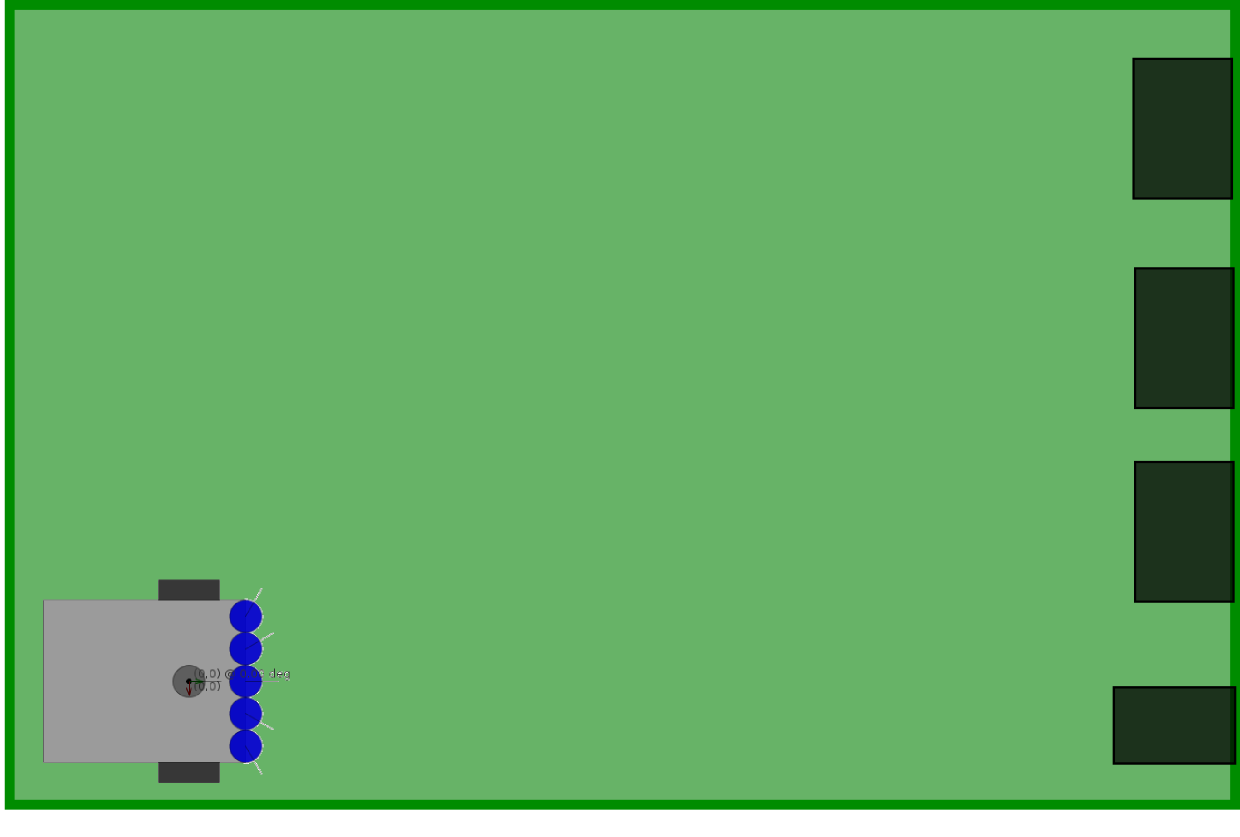
\includegraphics[width=0.6\textwidth]{./figuras/testes/teste1/layout.png}
	\caption{\textit{Layout} do ambiente do primeiro teste.}
	\label{fig:teste1_layout}
\end{figure}

\begin{figure}[H]
	\centering
	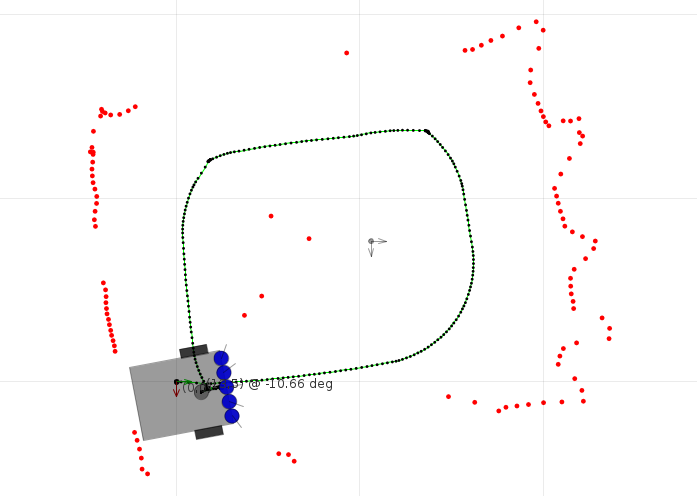
\includegraphics[width=0.9\textwidth]{./figuras/testes/teste1/mapa_encoders.png}
	\caption{Mapa gerado no primeiro teste a partir dos dados dos encoders usando filtragem por média móvel de 3 períodos para sensores IR.}
	\label{fig:teste1_mapa_encoders}
\end{figure}

\begin{figure}[H]
	\centering
	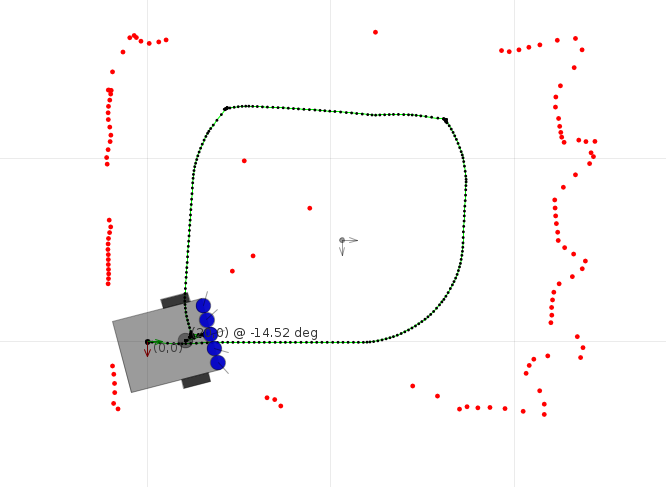
\includegraphics[width=0.8\textwidth]{./figuras/testes/teste1/mapa_encoders_giro.png}
	\caption{Mapa gerado no primeiro teste a partir dos dados dos encoders, com correção de erros pelo giroscópio ($L_\omega = 0.0025 \unit{rad/s}$) e filtragem por média móvel de 3 períodos para sensores IR.}
	\label{fig:teste1_mapa_encoders_giro}
\end{figure}

\begin{figure}[H]
	\centering
	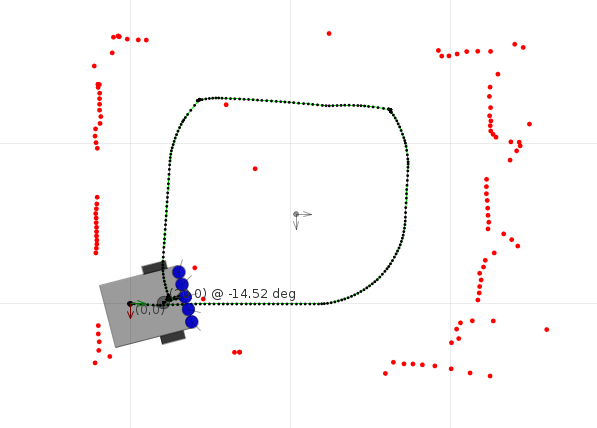
\includegraphics[width=0.8\textwidth]{./figuras/testes/teste1/mapa_encoders_giro_media0.png}
	\caption{Mapa gerado no primeiro teste a partir dos dados dos encoders, com correção de erros pelo giroscópio ($L_\omega = 0.0025 \unit{rad/s}$) sem filtragem por média móvel dos sensores IR.}
	\label{fig:teste1_mapa_encoders_giro_media0}
\end{figure}

\begin{figure}[H]
	\centering
	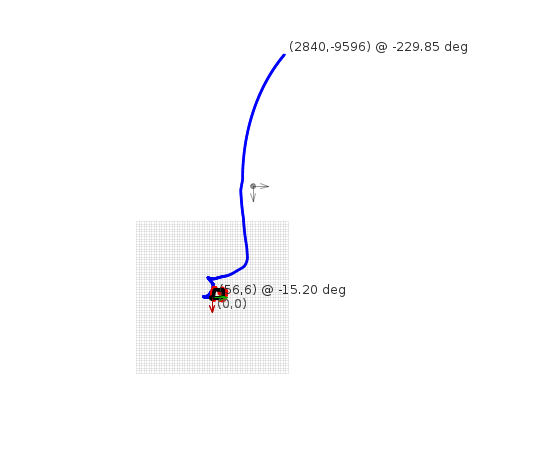
\includegraphics[width=0.8\textwidth]{./figuras/testes/teste1/mapa_acelerometro.png}
	\caption{Trilha do robô (em azul) no primeiro teste calculada somente a partir dos dados do acelerômetro e do giroscópio.}
	\label{fig:teste1_mapa_acelerometro}
\end{figure}

\begin{figure}[H]
	\centering
	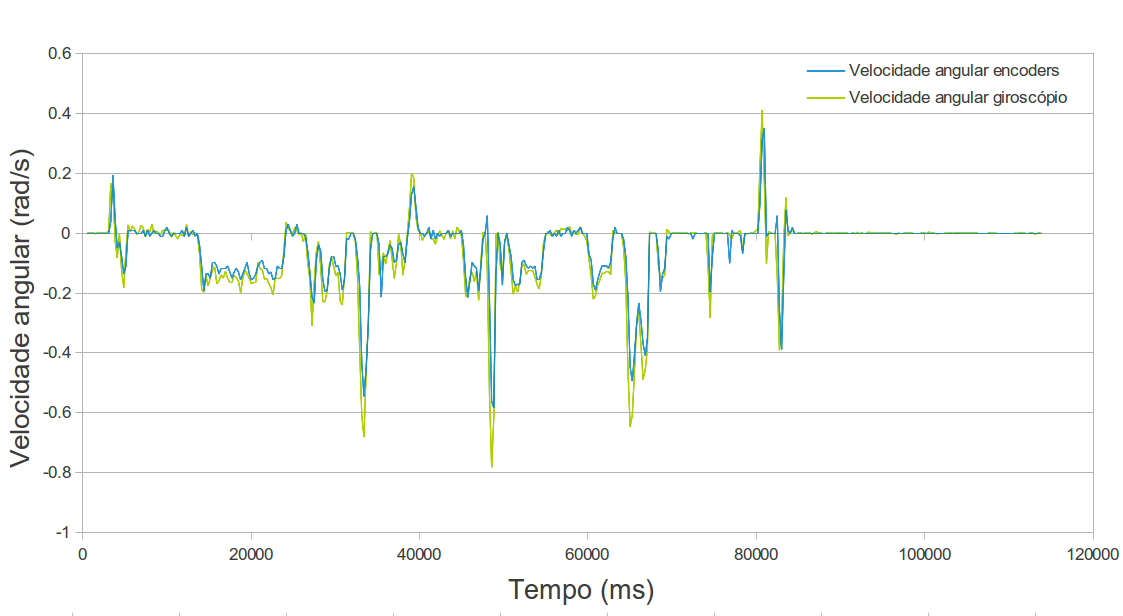
\includegraphics[width=1\textwidth]{./figuras/testes/teste1/grafico_giro.png}
	\caption{Gráfico comparativo de velocidades angulares obtidas no primeiro teste.}
	\label{fig:teste1_giro_grafico}
\end{figure}

\begin{figure}[H]
	\centering
	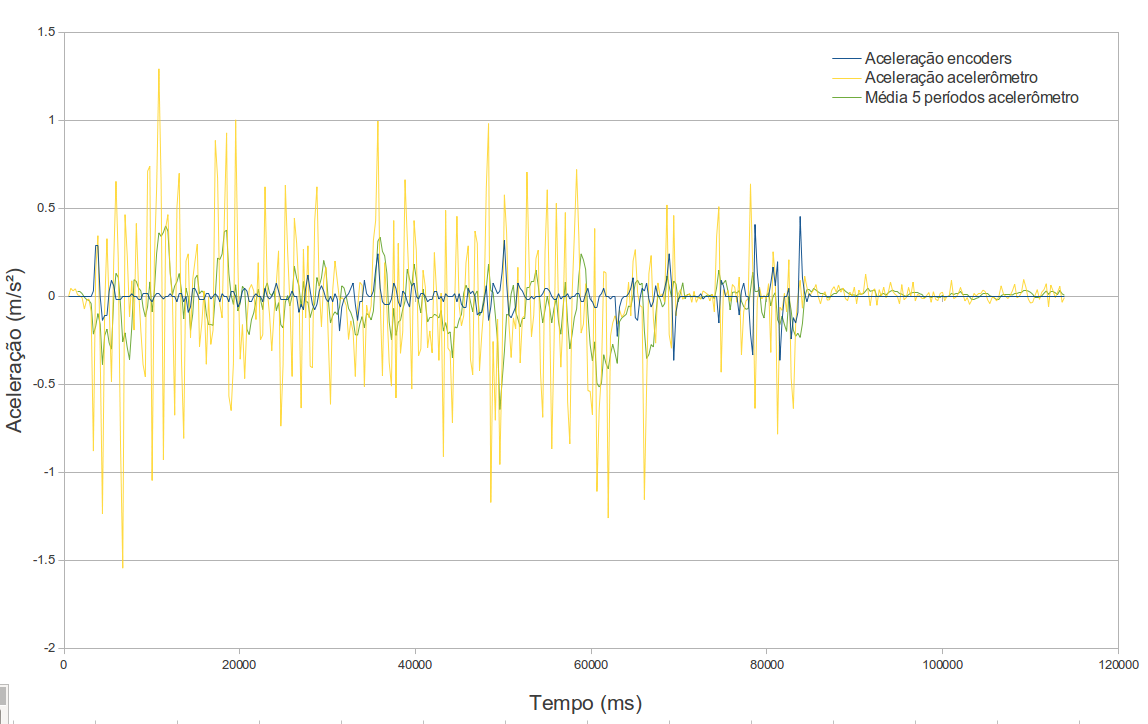
\includegraphics[width=1\textwidth]{./figuras/testes/teste1/grafico_acel.png}
	\caption{Gráfico comparativo de acelerações obtidas no primeiro teste.}
	\label{fig:teste1_acel_grafico}
\end{figure}



\section{Segundo teste}

O segundo teste foi realizado em um corredor de 2,25m de largura, no ambiente da Figura \ref{fig:teste2_foto}. A mochila que pode ser vista na foto foi posicionada no centro do corredor para que a detecção dela fosse feita pelo robô. Na Figura \ref{fig:teste2_mapa_encoders}, está presente o mapa produzido apenas com dados dos encoders. Vê-se que eles sofreram erros de medição nas curvas. Na Figura \ref{fig:teste2_mapa_encoders_giro}, pode-se ver um mapa produzido com correções desses erros pelo giroscópio, usando um limiar $L_\omega = 0.0025 \unit{rad/s}$. 

Nos mapas das Figuras \ref{fig:teste2_mapa_encoders} e \ref{fig:teste2_mapa_encoders_giro}, não foi utilizado nenhum tipo de filtragem (além do passa-faixa de 30 a 150cm) para os sensores infra-vermelhos. O uso de média móvel de 3 períodos (Figura \ref{fig:teste2_mapa_encoders_giro_media3}) não resultou em diferenças muito consideráveis, e a de 8 períodos (Figura \ref{fig:teste2_mapa_encoders_giro_media8}) gerou resultados visivelmente piores.

Percebe-se nesse teste, novamente, que o giroscópio foi confiável nas medições de velocidade angular. Já o acelerômetro, assim como no teste anterior, não pôde ser utilizado para correção de erros (pelos mesmos motivos já apresentados). A Figura \ref{fig:teste2_mapa_acelerometro} expôe a trilha do robô gerada apenas com os dados do acelerômetro e do giroscópio. Percebe-se que os resultados obtidos com o acelerômetro saem bastante da realidade.

\begin{figure}[H]
	\centering
	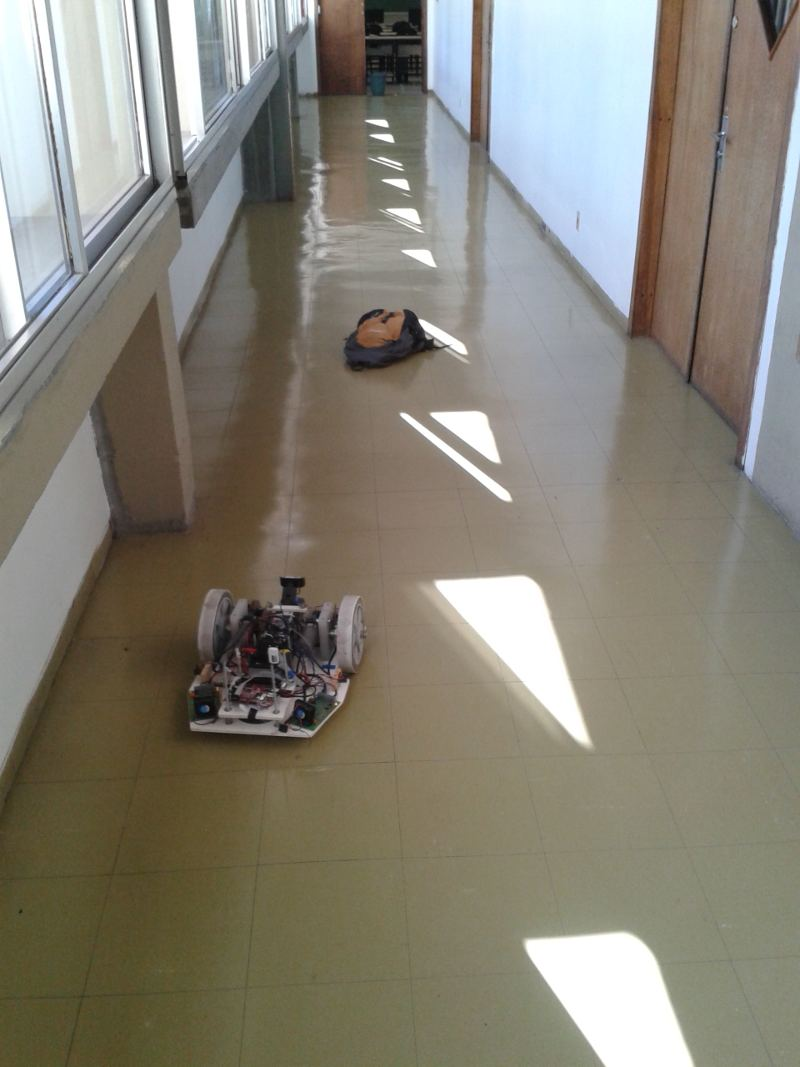
\includegraphics[width=0.9\textwidth]{./figuras/testes/teste2/foto_ambiente.jpg}
	\caption{Ambiente utilizado no segundo teste.}
	\label{fig:teste2_foto}
\end{figure}

\begin{figure}[H]
	\centering
	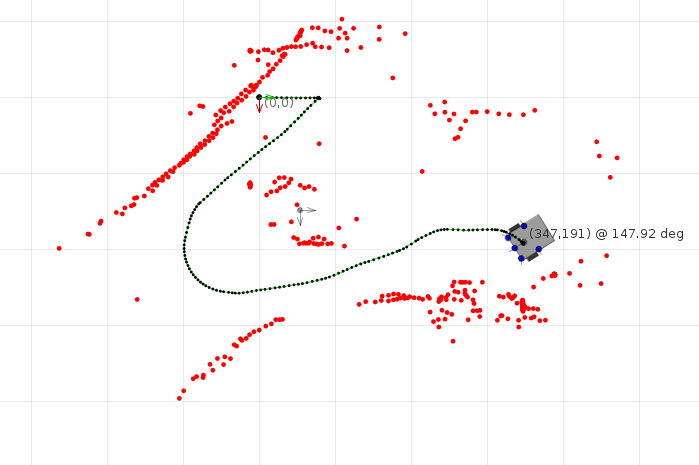
\includegraphics[width=0.9\textwidth]{./figuras/testes/teste2/mapa_encoders.png}
	\caption{Mapa gerado no segundo teste a partir dos dados dos encoders.}
	\label{fig:teste2_mapa_encoders}
\end{figure}

\begin{figure}[H]
	\centering
	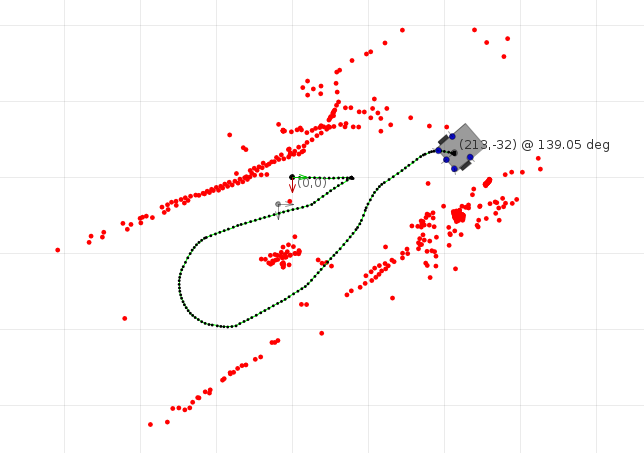
\includegraphics[width=0.9\textwidth]{./figuras/testes/teste2/mapa_encoders_giro.png}
	\caption{Mapa gerado no segundo teste a partir dos dados dos encoders, com correção de erros pelo giroscópio ($L_\omega = 0.0025 \unit{rad/s}$).}
	\label{fig:teste2_mapa_encoders_giro}
\end{figure}

\begin{figure}[H]
	\centering
	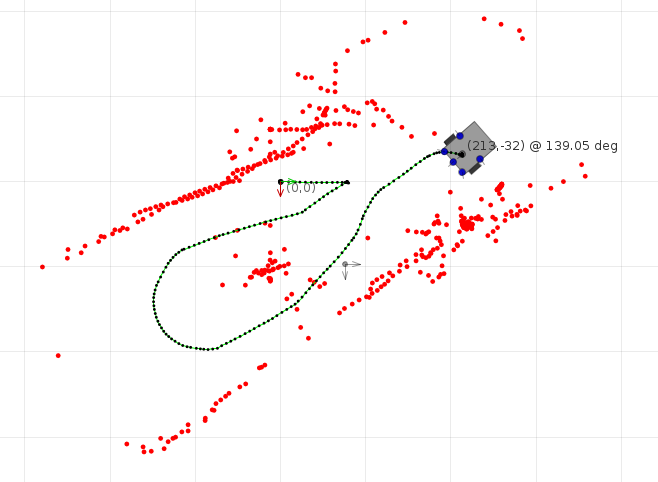
\includegraphics[width=0.9\textwidth]{./figuras/testes/teste2/mapa_encoders_giro_media3.png}
	\caption{Mapa gerado no primeiro teste a partir dos dados dos encoders, com correção de erros pelo giroscópio ($L_\omega = 0.0025 \unit{rad/s}$) e filtragem por média móvel de 3 períodos para sensores IR.}
	\label{fig:teste2_mapa_encoders_giro_media3}
\end{figure}

\begin{figure}[H]
	\centering
	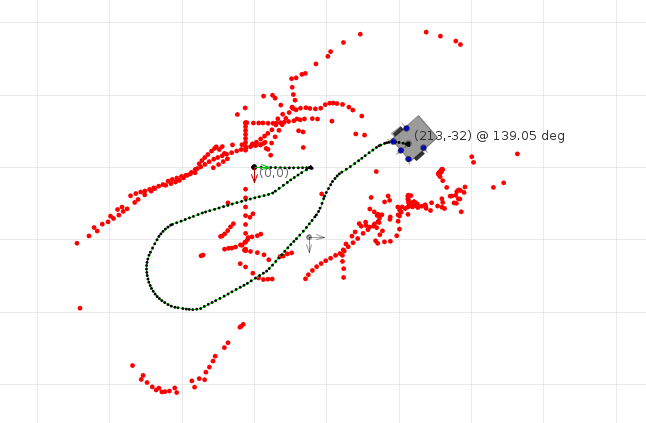
\includegraphics[width=0.9\textwidth]{./figuras/testes/teste2/mapa_encoders_giro_media8.png}
	\caption{Mapa gerado no primeiro teste a partir dos dados dos encoders, com correção de erros pelo giroscópio ($L_\omega = 0.0025 \unit{rad/s}$) e filtragem por média móvel de 8 períodos para sensores IR.}
	\label{fig:teste2_mapa_encoders_giro_media8}
\end{figure}

\begin{figure}[H]
	\centering
	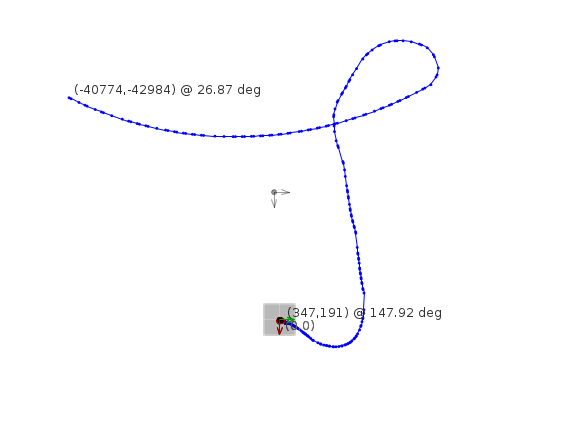
\includegraphics[width=0.8\textwidth]{./figuras/testes/teste2/mapa_acelerometro.png}
	\caption{Trilha do robô (em azul) no segundo teste calculada somente a partir dos dados do acelerômetro e do giroscópio.}
	\label{fig:teste2_mapa_acelerometro}
\end{figure}

\begin{figure}[H]
	\centering
	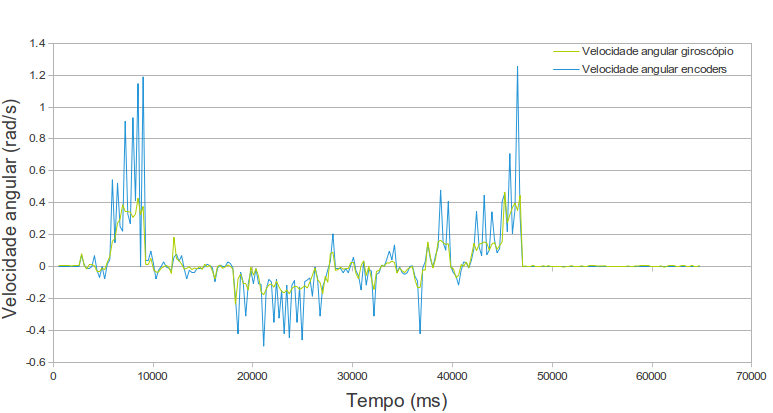
\includegraphics[width=1\textwidth]{./figuras/testes/teste2/grafico_giro.png}
	\caption{Gráfico comparativo de velocidades angulares obtidas no segundo teste.}
	\label{fig:teste2_giro_grafico}
\end{figure}

\begin{figure}[H]
	\centering
	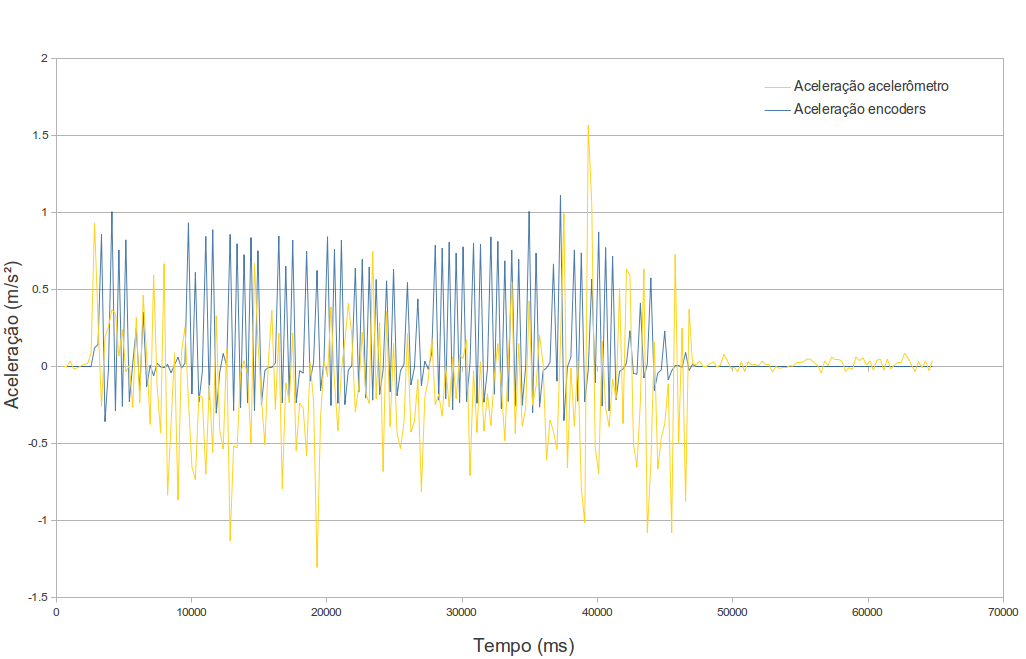
\includegraphics[width=1\textwidth]{./figuras/testes/teste2/grafico_acel.png}
	\caption{Gráfico comparativo de acelerações obtidas no segundo teste.}
	\label{fig:teste2_acel_grafico}
\end{figure}

\section{Terceiro teste}

O terceiro teste foi realizado partindo-se de um corredor de 2,25m de largura (à direita na Figura), saindo dele e voltando ao ponto de partida novamente. O ambiente está representado na Figura \ref{fig:teste3_foto}. Na Figura \ref{fig:teste3_mapa_encoders}, está presente o mapa produzido apenas com dados dos encoders. Vê-se que eles sofreram erros de medição nas curvas, assim como no teste anterior. Na Figura \ref{fig:teste3_mapa_encoders_giro}, pode-se ver um mapa produzido com correções desses erros pelo giroscópio, usando um limiar $L_\omega = 0.0025 \unit{rad/s}$.

Nos mapas das Figuras \ref{fig:teste3_mapa_encoders} e \ref{fig:teste3_mapa_encoders_giro}, não foi utilizado nenhum tipo de filtragem (além do passa-faixa de 30 a 150cm) para os sensores infra-vermelhos. O uso de média móvel de 5 períodos (Figura \ref{fig:teste3_mapa_encoders_giro_media5}), a melhor configuração encontrada, resultou em leves melhorias na qualidade do mapa.

Percebe-se nesse teste, novamente, que o giroscópio foi confiável nas medições de velocidade angular. Já o acelerômetro, assim como nos testes anteriores, não pôde ser utilizado para correção de erros (pelos mesmos motivos já apresentados). A Figura \ref{fig:teste3_mapa_acelerometro} expôe a trilha do robô gerada apenas com os dados do acelerômetro e do giroscópio. Percebe-se novamente que os resultados obtidos com o acelerômetro fogem bastante da realidade.

\begin{figure}[H]
	\centering
	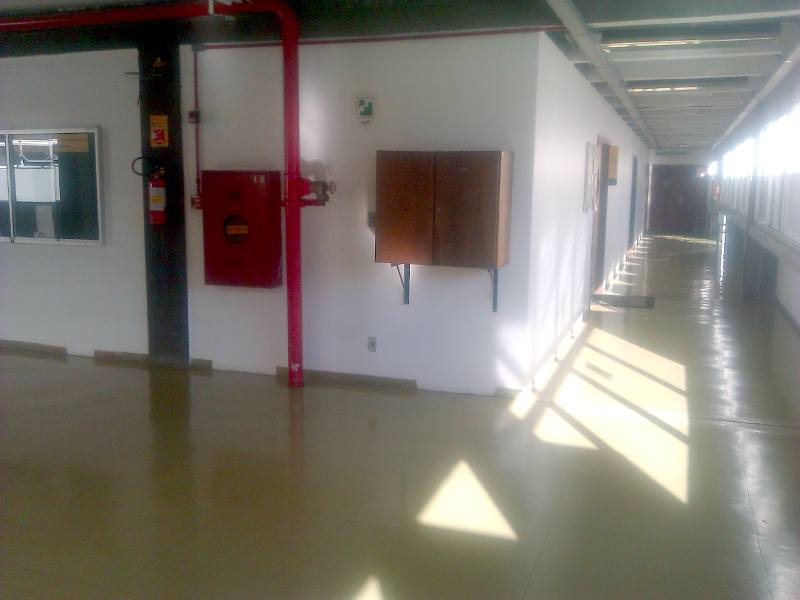
\includegraphics[width=0.7\textwidth]{./figuras/testes/teste3/foto_ambiente.jpg}
	\caption{Ambiente utilizado no terceiro teste.}
	\label{fig:teste3_foto}
\end{figure}

\begin{figure}[H]
	\centering
	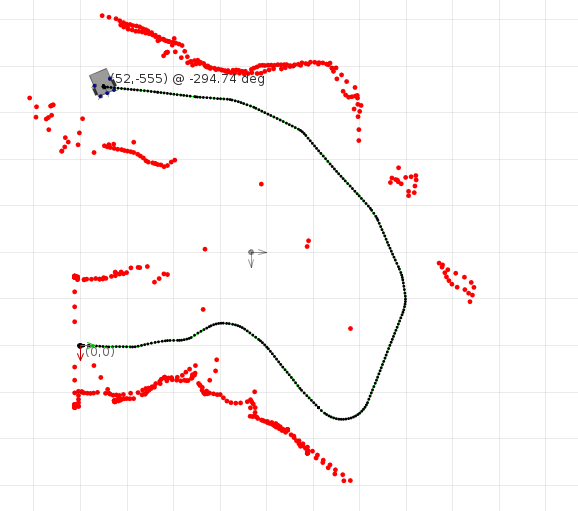
\includegraphics[width=0.9\textwidth]{./figuras/testes/teste3/mapa_encoders.png}
	\caption{Mapa gerado no terceiro teste a partir dos dados dos encoders.}
	\label{fig:teste3_mapa_encoders}
\end{figure}

\begin{figure}[H]
	\centering
	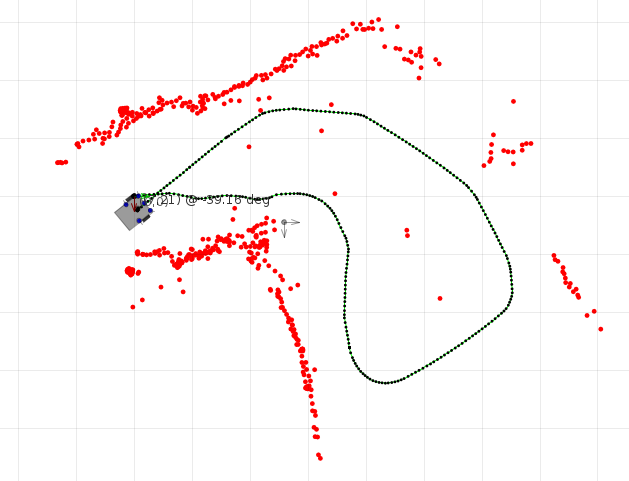
\includegraphics[width=0.8\textwidth]{./figuras/testes/teste3/mapa_encoders_giro.png}
	\caption{Mapa gerado no terceiro teste a partir dos dados dos encoders, com correção de erros pelo giroscópio ($L_\omega = 0.0025 \unit{rad/s}$).}
	\label{fig:teste3_mapa_encoders_giro}
\end{figure}

\begin{figure}[H]
	\centering
	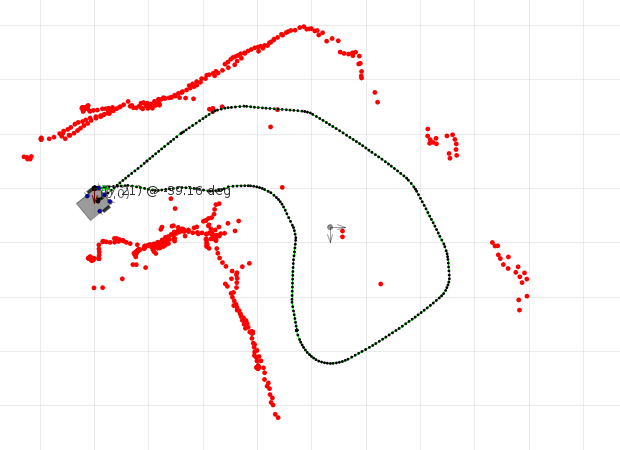
\includegraphics[width=0.8\textwidth]{./figuras/testes/teste3/mapa_encoders_giro_media5.png}
	\caption{Mapa gerado no primeiro teste a partir dos dados dos encoders, com correção de erros pelo giroscópio ($L_\omega = 0.0025 \unit{rad/s}$) e filtragem por média móvel de 5 períodos para sensores IR.}
	\label{fig:teste3_mapa_encoders_giro_media5}
\end{figure}

\begin{figure}[H]
	\centering
	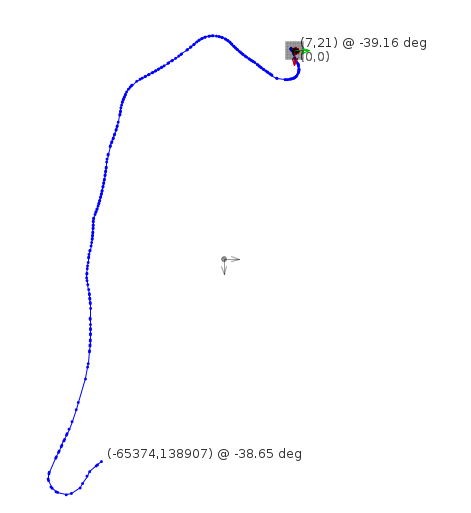
\includegraphics[width=0.8\textwidth]{./figuras/testes/teste3/mapa_acelerometro.png}
	\caption{Trilha do robô (em azul) no terceiro teste calculada somente a partir dos dados do acelerômetro e do giroscópio.}
	\label{fig:teste3_mapa_acelerometro}
\end{figure}

\begin{figure}[H]
	\centering
	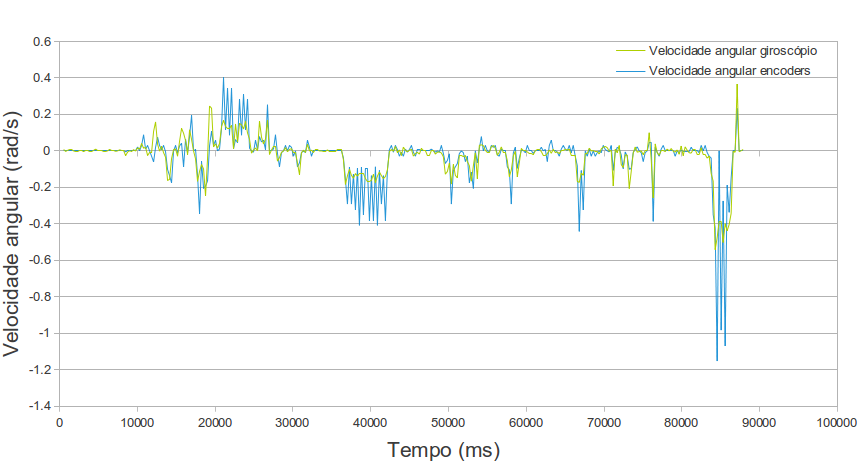
\includegraphics[width=1\textwidth]{./figuras/testes/teste3/grafico_giro.png}
	\caption{Gráfico comparativo de velocidades angulares obtidas no terceiro teste.}
	\label{fig:teste3_giro_grafico}
\end{figure}

\begin{figure}[H]
	\centering
	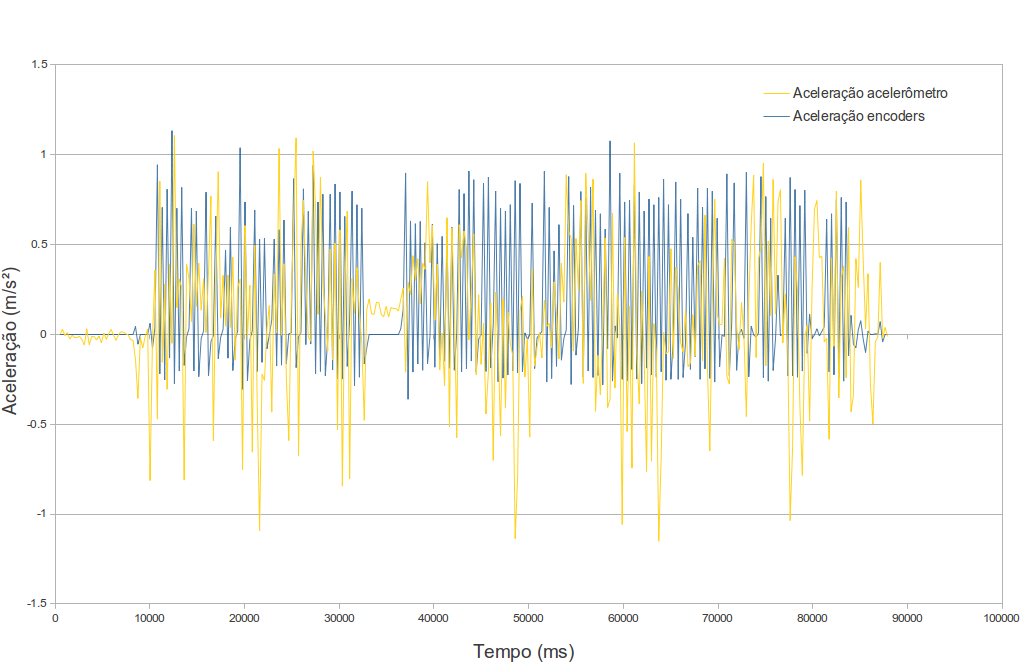
\includegraphics[width=1\textwidth]{./figuras/testes/teste3/grafico_acel.png}
	\caption{Gráfico comparativo de acelerações obtidas no terceiro teste.}
	\label{fig:teste3_acel_grafico}
\end{figure}

\section{Quarto teste}

O quarto teste foi realizado na extensão do corredor principal do terceiro andar dos blocos A, B, C e D da UTFPR campus Curitiba. O ambiente está representado na Figura \ref{fig:teste4_foto}. Um mapa produzido apenas com dados dos encoders está explicitado na Figura \ref{fig:teste4_mapa_encoders}. Vê-se que os encoders sofreram erros de medição, pois o mapa aparece de forma curvada. Na Figura \ref{fig:teste4_mapa_encoders_giro}, pode-se ver um mapa produzido com correções desses erros pelo giroscópio, usando um limiar $L_\omega = 0.003 \unit{rad/s}$.

Nos mapas das Figuras \ref{fig:teste4_mapa_encoders} e \ref{fig:teste4_mapa_encoders_giro}, não foi utilizado nenhum tipo de filtragem (além do passa-faixa de 30 a 150cm) para os sensores infra-vermelhos. O uso de média móvel de 4 períodos (Figura \ref{fig:teste4_mapa_encoders_giro_media4}), a melhor configuração encontrada, resultou em leves melhorias na qualidade do mapa.

Percebe-se nesse teste, novamente, que o giroscópio foi confiável nas medições de velocidade angular. Já o acelerômetro, assim como nos testes anteriores, não pôde ser utilizado para correção de erros pelos mesmos motivos já apresentados. %A Figura \ref{fig:teste4_mapa_acelerometro} expôe a trilha do robô gerada apenas com os dados do acelerômetro e do giroscópio. Percebe-se novamente que os resultados obtidos fogem muito da realidade.

\begin{figure}[H]
	\centering
	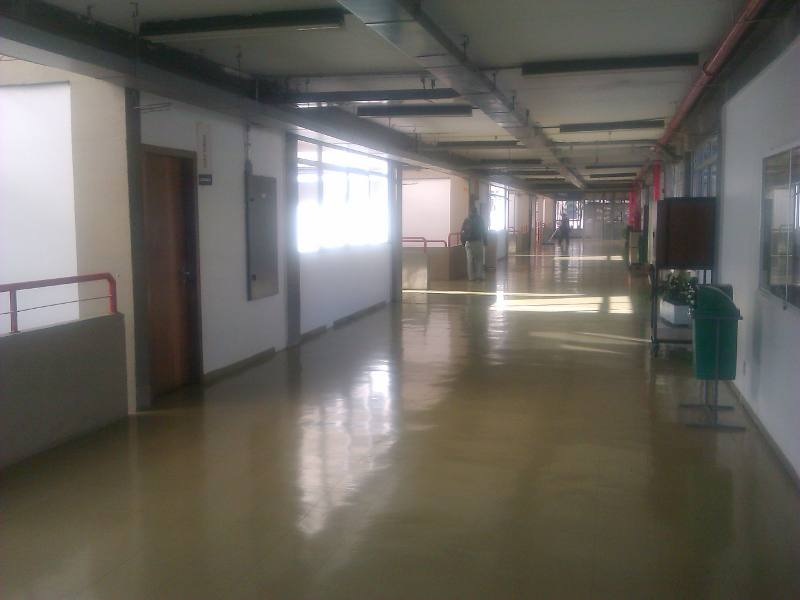
\includegraphics[width=0.7\textwidth]{./figuras/testes/teste4/foto_ambiente.jpg}
	\caption{Ambiente utilizado no quarto teste.}
	\label{fig:teste4_foto}
\end{figure}

\begin{figure}[H]
	\centering
	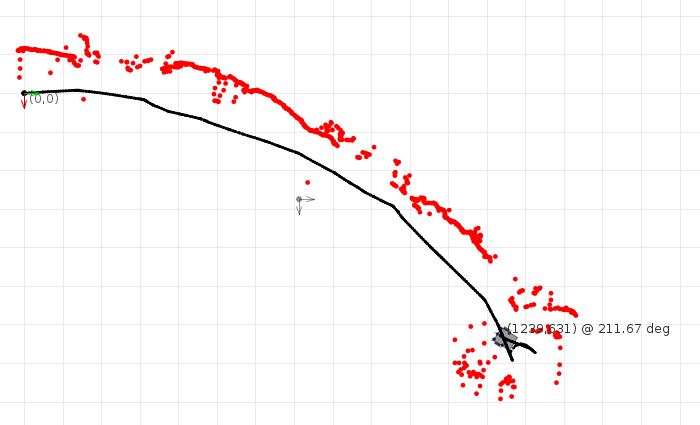
\includegraphics[width=1\textwidth]{./figuras/testes/teste4/mapa_encoders.png}
	\caption{Mapa gerado no quarto teste a partir dos dados dos encoders.}
	\label{fig:teste4_mapa_encoders}
\end{figure}

\begin{figure}[H]
	\centering
	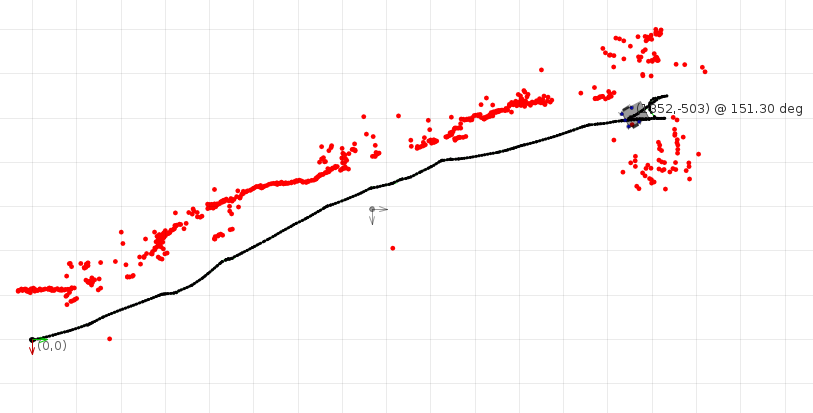
\includegraphics[width=1\textwidth]{./figuras/testes/teste4/mapa_encoders_giro.png}
	\caption{Mapa gerado no quarto teste a partir dos dados dos encoders, com correção de erros pelo giroscópio ($L_\omega = 0.003 \unit{rad/s}$).}
	\label{fig:teste4_mapa_encoders_giro}
\end{figure}

\begin{figure}[H]
	\centering
	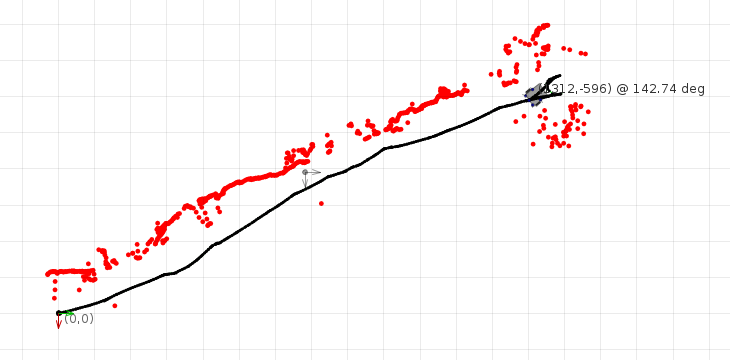
\includegraphics[width=1\textwidth]{./figuras/testes/teste4/mapa_encoders_giro_media4.png}
	\caption{Mapa gerado no primeiro teste a partir dos dados dos encoders, com correção de erros pelo giroscópio ($L_\omega = 0.003 \unit{rad/s}$) e filtragem por média móvel de 4 períodos para sensores IR.}
	\label{fig:teste4_mapa_encoders_giro_media4}
\end{figure}

\begin{figure}[H]
	\centering
	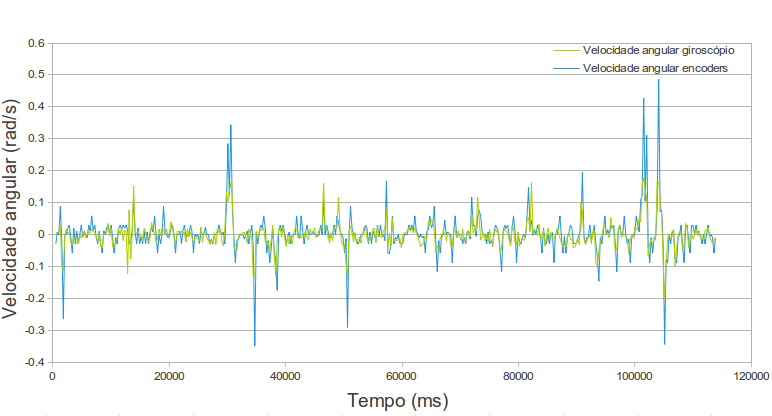
\includegraphics[width=1\textwidth]{./figuras/testes/teste4/grafico_giro.png}
	\caption{Gráfico comparativo de velocidades angulares obtidas no quarto teste.}
	\label{fig:teste4_giro_grafico}
\end{figure}

\begin{figure}[H]
	\centering
	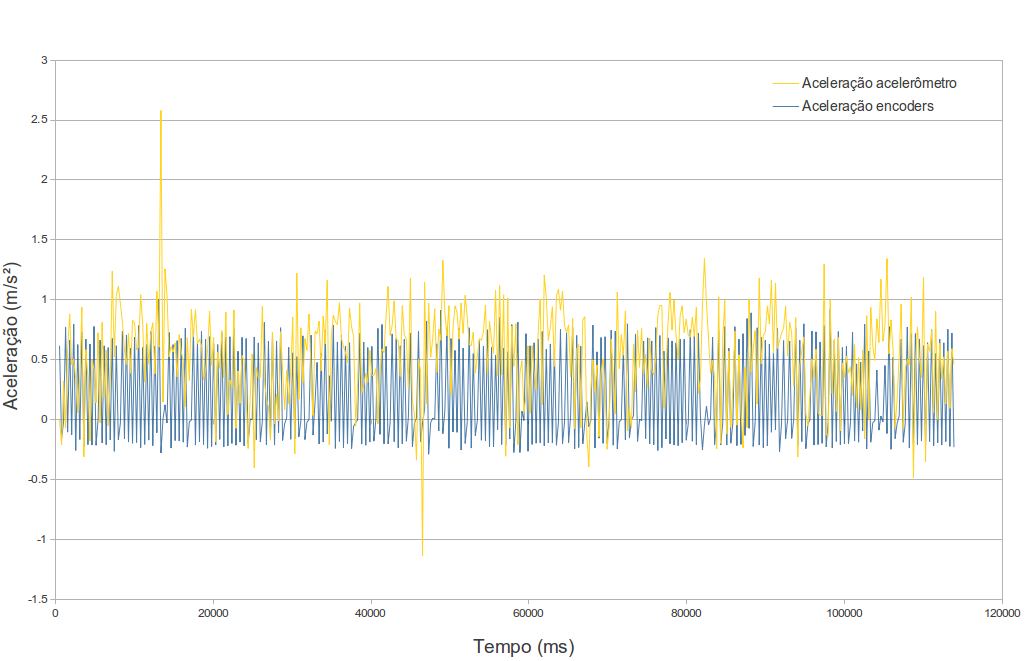
\includegraphics[width=1\textwidth]{./figuras/testes/teste4/grafico_acel.png}
	\caption{Gráfico comparativo de acelerações obtidas no quarto teste.}
	\label{fig:teste4_acel_grafico}
\end{figure}

\chapter{Conclusões}

Pôde ser visto nos testes apresentados que os encoders sofreram falhas nas medidas, sobretudo na realização de curvas. Outro aspecto percebido também pela equipe é que erros de medição ocorrem frequentemente quando o robô inicia o movimento de uma roda parada, ou quando inverte o sentido de rotação abruptamente. Uma das possíveis causas dos erros podem ser os discos dos encoders, que estão visivelmente danificados em certos pontos. Eles deveriam gerar, nominalmente, 1800 pulsos por volta, mas geram na prática aproximadamente 1600 pulsos.
Outra causa provável é que a correia utilizada para fazer o acoplamento do eixo da roda com o eixo do encoder é de borracha, e frequentemente está sujeita a escorregamentos. A equipe efetou tentativas de reduzir esse problema utilizando uma polia maior (e com mais aderência) no eixo dos encoders, e aumentando a aderência do eixo das rodas aplicando a ele uma fita de borracha. Porém, ainda sim os problemas persistiram. 

Uma alternativa viável seria utilizar outro disco para os encoders, com menos pulsos por volta e que sejam menos sucetíveis a falhas de leitura. Além disso, para acoplar o encoder às rodas, uma solução pode ser a utilização de uma correia dentada, que é menos sujeita a escorregamentos que uma correia de borracha. Outra opção seria acoplar os discos dos encoders diretamente ao eixo das rodas, dessa maneira eliminando o problema das correias.

Um aspecto que foi bem-sucedido nos testes foi a utilização do giroscópio para a correção de erros dos encoders. Sobretudo o giroscópio foi de grande valia para determinar com maior exatidão a orientação do robô na realização de curvas. Um aspecto interessante que pode ser trabalhado em projetos futuros é a determinação do limiar $L_\omega$ para cada caso específico. Nos testes aqui apresentados, o valor foi determinado empiricamente em cada teste, mas seria interessante que houvesse um trabalho no desenvolvimento de um algoritmo para determinar dinamicamente o valor de $L_\omega$, adequando-o a cada caso. Possivelmente o filto de Kalman seja outra opção para corrigir os erros dinamicamente. Porém, conhecidamente, a complexidade de utilização dele na prática é considerável.

Percebeu-se que o acelerômetro não foi eficaz para o fim de correção de erros de odometria, ao menos não da forma como os dados estão sendo atualmente obtidos e tratados. A obtenção de dados é feita a partir de amostras instantâneas a 3.89 Hz. No escopo do projeto (tendo em vista as limitações de tempo) não foi possível trabalhar mais à fundo com os dados do acelerômetro. Porém, deixa-se a possibilidade para trabalhos futuros. Como alternativa de tratamento desses dados, possivelmente possa ser utilizada uma taxa de amostragem maior para o acelerômetro, utilizando um processo de filtragem para reduzir os ruídos da aceleração.

Do ponto de vista dos objetivos, percebe-se que a maioria deles foram alcançados. Foi implementado com sucesso um \textit{software} com interface gráfica para geração e visualização de mapas, visualização de imagens da \textit{webcam} do robô e controle do robô por meio do teclado. A comunicação foi implementada satisfatoriamente, tanto entre a estação base e a placa TS-7260 (via Wi-Fi) quanto entre a TS e a placa de baixo nível, via porta serial. Uma \textit{webcam} USB foi instalada e configurada com sucesso no robô para a transmissão de imagens ao usuário. O giroscópio foi utilizado satisfatoriamente na prática para corrigir erros de leituras dos encoders e escorregamento das rodas. Uma placa de circuito impresso, de tamanho reduzido, foi desenvolvida de forma a integrar as funções de baixo nível do robô: interface com os encoders, sensores infra-vermelhos, acelerômetro e giroscópio, e geração de PWM para os motores.

Como última consideração, enfatiza-se que este projeto não chegou ao seu fim, mas pelo contrário, um novo caminho foi aberto para pesquisas mais aprofundadas no que tange o mapeamento 2D de ambientes. A possibilidade está aberta a novas equipes para utilizarem a plataforma de mapeamento desenvolvida para o Bellator -- o que envolve tanto o \textit{hardware} quanto o \textit{software}. Apesar deste trabalho ter sido consideravelmente extenso e demandar muito tempo e energia de todos os membros da equipe, pode-se dizer que com ele o ponta-pé inicial foi dado, e que ainda existem muitas possibilidades a serem pensadas e realizadas para o futuro.


%Em termos matemáticos:
%\begin{equation}
%  \overrightarrow{P_C} = \overrightarrow{P}
%  \label{eq:IR-P_C}
%\end{equation}
%\begin{eqnarray*}
%  |\overrightarrow{P_1}| &=&  \overrightarrow{P_{IR}}\\
%  \phi(\overrightarrow{P_1}) &=& \theta
%  \label{eq:IR-P_!}
%\end{eqnarray*}
%


